\documentclass[letterpaper,twocolumn,10pt]{article}
\usepackage{usenix-2020-09}
\usepackage{amsmath}
\usepackage{amssymb}
\usepackage{booktabs}
\usepackage{graphicx}
\usepackage{tabularx}
\usepackage{multirow}
\usepackage{xspace}

\newcommand{\sys}{\textsc{slangGraph}\xspace}
\newcommand{\code}[1]{\texttt{#1}}

\begin{document}
\date{}
\title{\Large \bf slangGraph: From Tool Calls to Kernel Boundaries\\
  Composable, Evidence-Carrying Enforcement for LLM Agents}
\author{Anonymous submission}
\maketitle

\begin{abstract}
Tool-using language-model agents execute attacker-influenced actions with the
authority of conventional software. Existing defenses primarily decide whether
a proposed tool call is acceptable. That boundary is insufficient when wrappers
can be bypassed, a tool rewrites its arguments, or an admitted implementation
uses undeclared files, processes, or channels.

We present \sys, an LSM-inspired security architecture integrated into
LangGraph. A constructive, tool-authored discretionary policy proposes concrete
authority; independently developed mandatory modules may only remove authority.
The framework converts the result into a platform-neutral grant, expands it into
exact enforcement obligations, conservatively assigns those obligations to host,
service, and resource adapters, and releases a worker only after verifying
worker-bound activation evidence. Its Linux backend executes hostile Python
tools in fresh bubblewrap workers with explicit mounts, namespaces, seccomp,
resource limits, bounded data-only results, and termination-aware flow state.

Across eight vulnerable tools, deterministic canaries show that call-boundary
defenses can approve calls whose implementations reach unauthorized sinks. The
accepted Linux contract passes 55 focused kernel and flow tests and the complete
518-test upstream-compatible suite. Matched microbenchmarks show 13.2\% overhead
for capability-only mediation and 49.0\% for five modules. \sys does not infer
user intent or claim automatic noninterference; it makes authorized authority,
its enforcing components, and activation evidence explicit.
\end{abstract}

\section{Introduction}

Language-model agents turn text into effects. A model can select a tool, provide
arguments, consume its result, and continue across retries, checkpoints,
subagents, and parallel branches. Indirect prompt injection makes the model's
control decisions attacker-influenced~\cite{greshake2023indirect,agentdojo,
injecagent}. The security problem is therefore not only whether the model emits
a syntactically suspicious call. It is whether the resulting computation can
exercise authority that was not explicitly authorized.

Recent systems make major advances at the agent--tool interface. Progent checks
symbolic rules over tool names and arguments and verifies monotonic policy
updates~\cite{progent}. SEAgent applies mandatory access control over an
information-flow graph~\cite{seagent}. CaMeL separates control from untrusted
data and uses capabilities to protect data flows~\cite{camel}. These systems
improve policy expressiveness or model-level data-flow integrity. Yet an
interface decision does not by itself constrain the implementation below the
interface. A policy may approve \code{read\_file("reports/q3")}, after which a
hostile implementation resolves a different path, imports a dependency with a
side effect, opens an ambient socket, or spawns a helper. Likewise, an outer
middleware guard does not mediate an execution callback that a wrapper invokes
twice with different arguments.

Operating systems encountered the analogous problem decades ago. Linux Security
Modules (LSM) separates fixed mediation hooks from the policies loaded behind
them, preserves discretionary checks, lets multiple mandatory modules restrict
an operation, and attaches private security state to protected
objects~\cite{wright2002lsm,linuxlsm}. The analogy is useful, but agents add three
complications. First, policy must describe semantic resources such as recipients
and SQL operations, not just kernel objects. Second, enforcement may be split
among a local sandbox, a service broker, and a resource-side credential issuer.
Third, a decision is not evidence that those mechanisms were installed for the
worker that executed the tool.

This paper presents \sys, an LSM-inspired security framework implemented as a
fork of LangGraph. The design follows a strict separation:

\begin{quote}
\emph{Authorization determines what should happen. Enforcement adapters bound
what can happen. Evidence establishes which bounds were active.}
\end{quote}

The framework does not infer security policy from model behavior. A tool author
constructively requests authority; the principal's envelope and shares intersect
that request; mandatory modules can only subtract. The surviving rules form an
immutable, platform-neutral \emph{grant}. Every rule and the closed-world runtime
baseline become exact obligations. Adapters must implement each obligation
exactly or more restrictively, declare their dependencies, and return
worker-bound activation evidence. An unsupported rule denies instead of being
approximated by a broad capability class.

Our current reference backend makes this contract operational for mediated local
Python tools on Linux. It supports regular-file and live directory-subtree access
plus explicitly named resource ceilings. Network, remote-service, credential,
delegation, and executable authority are rejected by this backend; the generic
grant and adapter contracts are designed for additional backends. This is a
deliberately narrower but stronger claim than process-wide MAC or complete agent
noninterference.

This work makes four contributions:

\begin{itemize}
  \item We identify the \emph{authorization--enforcement gap}: expressive
  call-boundary policies do not constrain hostile implementations or establish
  that an enforcement mechanism was active.
  \item We design a composable policy pipeline combining tool-authored DAC,
  restrictive mandatory modules, exact grants, an obligation DAG, conservative
  adapter lowering, and activation evidence.
  \item We implement innermost mediation in LangGraph and a Linux executor that
  confines each admitted Python tool before importing untrusted code.
  \item We evaluate mediation exposure, deterministic bypass canaries, Linux
  contract failures, compatibility, and policy-path overhead. Our results show
  both where interface defenses are strong and where only active confinement
  supports the claimed boundary.
\end{itemize}

\section{Problem and Goals}
\label{sec:problem}

\subsection{The authorization--enforcement gap}

Let a proposed call be $c=(p,t,a,h)$: authenticated principal $p$, tool $t$,
arguments $a$, and prior security history $h$. A call-boundary monitor computes
$D(c)\in\{\mathsf{allow},\mathsf{deny}\}$. For benign tools, $D$ can be an
effective enforcement point. For hostile tools, however, the actual effect set
$E(t,a)$ is not necessarily a function of the declared descriptor. The desired
property is not merely $D(c)=\mathsf{allow}$, but

\begin{equation}
  E(t,a) \subseteq A(c),
  \label{eq:subset}
\end{equation}

where $A(c)$ is the exact authorized authority, including runtime requirements.
Equation~\ref{eq:subset} cannot be established by trusting $t$'s metadata. It
requires an enforcement mechanism whose effective authority is a subset of the
grant and evidence that the mechanism protected this execution.

Three examples expose the distinction. A path policy can approve a relative path
before the implementation joins it with an attacker-controlled base directory.
A URL policy can approve HTTPS while the implementation accepts \code{file://}.
A mail tool can validate the first recipient while its implementation sends a
larger list. These are not necessarily failures of the policy language: they are
failures to keep resource resolution and effects below the mediation point.

\subsection{Design goals}

\paragraph{G1: enforcement over inference.}
Descriptors, model reasoning, and static analysis help construct policy, but are
not evidence of runtime behavior. The system must bound effects of hostile code.

\paragraph{G2: policy composition without grant paths.}
Tools propose DAC; operator modules impose mandatory restrictions. No module,
ordering choice, transform, or delegation may turn a prior denial into authority.

\paragraph{G3: portable policy, replaceable mechanisms.}
Policies name semantic operations and resources. Linux mounts, Windows handles,
service tokens, and sandbox bytecode belong in adapter plans, not the grant.

\paragraph{G4: exact negotiation and fail-closed lowering.}
Advertising ``network'' is insufficient. An adapter must state whether it can
enforce the concrete protocol, endpoint, method, resource scope, conditions, and
denial of unlisted authority. Unsupported requests deny.

\paragraph{G5: complete mediation within a declared boundary.}
Every physical execution through a configured \code{ToolNode} or
\code{guarded\_tool}, including retries and rewritten calls, must traverse the
same innermost check. The system must state what lies outside this boundary.

\paragraph{G6: evidence before release.}
A plan digest records intent, not installation. The coordinator releases
untrusted code only after trusted setup and independent observations bind the
actual worker, payload, grant, plan, and obligations.

\paragraph{Non-goals.}
\sys does not infer user intent, prove that an allowed action is beneficial,
protect unmediated arbitrary Python nodes, or automatically track all information
flows through model context and external storage. These properties require
task-specific authority, mediation of additional sinks, and conservative labels.

\section{Threat Model and Security Contract}
\label{sec:threat}

The adversary controls model outputs, tool arguments, retrieved data, tool
implementations, native tool dependencies after confinement, and subagent
prompts. It may exploit retries, argument rewriting, path races, dependency side
effects, malformed output, resource exhaustion, and failures during cancellation
or audit.

The trusted computing base (TCB) contains principal authentication and binding,
the coordinator, policy modules and backend, normalizers, grant compiler,
selected adapters, launcher, startup shim, interpreter startup, audit and flow
stores, and the underlying OS. A policy module affects authorization and is
therefore explicitly trusted. Tool-authored declarations are untrusted requests,
not facts.

The implemented Linux contract covers statically configured local Python tools
mediated by \code{ToolNode} or \code{guarded\_tool} and run in fresh workers.
It supports regular-file reads, live directory-subtree reads, exact-file
read/write/truncate, directory-subtree read/write/create/delete/truncate, and
explicit CPU, address-space, per-file-size, private-tmpfs, descriptor, process,
and wall-time limits. Filesystem grants describe live paths, not snapshots.
Special files and subtrees crossing nested host mounts are rejected.

The current backend excludes network and service access, dependency identity,
RSS and cgroup-memory quotas, aggregate persistent-storage quotas, and executable
authority. Calls requiring these guarantees deny before tool execution. Ordinary
graph nodes, model clients, callbacks, renderers, and unwrapped aliases are
outside the Linux worker boundary. They must be trusted or separately mediated.

We claim the following only for an execution reported \emph{enforced}: the
framework can identify its exact authorized authority; map every restriction to
an enforcing component; and provide authenticated, worker-bound evidence that
all required components were active before untrusted code ran. A degraded run,
an advisory waiver with unknown effective authority, or uncertain termination
does not receive this claim.

\section{Architecture}
\label{sec:architecture}

Figure~\ref{fig:pipeline} shows the path from intent to execution. The central
object is the grant, not a Linux sandbox profile.

\begin{figure*}[t]
\centering
\fbox{\begin{minipage}{0.96\textwidth}
\centering
\textbf{authenticated principal + normalized intent + tool profile}
$\longrightarrow$ constructive DAC candidate
$\longrightarrow$ restrictive mandatory filtering
$\longrightarrow$ immutable platform-neutral grant\\[3pt]
$\longrightarrow$ exact obligation DAG + closed-world baseline
$\longrightarrow$ host/service/resource adapter negotiation
$\longrightarrow$ conservative native plans\\[3pt]
$\longrightarrow$ trusted worker setup
$\longrightarrow$ activation receipt verification
$\longrightarrow$ release
$\longrightarrow$ execution
$\longrightarrow$ termination evidence
\end{minipage}}
\caption{The \sys authorization-to-enforcement pipeline. No plan or capability
class alone is evidence that enforcement is active.}
\label{fig:pipeline}
\end{figure*}

\subsection{Constructive DAC and restrictive MAC}

Each tool profile names an owner, callers, exact resource templates, syscall
profile, and \code{need}/\code{want} requirements. The principal has a typed
authority envelope; explicit shares may add resources delegated by another
owner. For normalized intent $i$, the DAC candidate is

\begin{equation}
 C(i)=P_t(i)\cap E_p\cap S_p,
\end{equation}

where $P_t$ is the tool's requested profile, $E_p$ the principal envelope, and
$S_p$ applicable shares. Undeclared tools receive no caller or resource
authority. A missing \code{need} descendant denies; an unavailable \code{want}
is removed rather than replaced with ambient access.

Mandatory modules receive typed requests and may emit attributed, bounded
forbid constraints or deny a call. The framework owns attribution, validates
entity references and complexity, and treats diagnostics as denial. It applies
each constraint to concrete grant lines and also evaluates forbidden
combinations over the whole candidate. This supports policies such as ``no
sensitive reads together with outbound communication,'' which cannot be checked
by evaluating each line independently. The current implementation ships a typed
reference backend. Cedar is a replaceable authorization backend because Cedar's
principal--action--resource--context model and forbid semantics suit this
stage~\cite{cedar}; Cedar syntax is not part of the grant or adapter API.

Only a trusted prepare hook may transform arguments. The framework renormalizes
the output, reruns DAC, and requires semantic authority to be unchanged or
narrower. String length or structural similarity is not used as an authority
ordering. Delegation similarly copies private module state and restricts scopes;
the exact-grant path compares typed authority.

\subsection{Platform-neutral grant}

The immutable grant binds the authenticated principal, exact tool artifact,
normalized intent, call identity, policy version, and rules. A rule contains a
typed action, semantic resource selector, conditions, source-line provenance,
and requirement identity. Runtime dependencies---interpreter roots, environment
values, descriptors, and protocol channels---are operator-owned baseline rules,
not authority an adapter may add for itself.

The grant is a closed-world allowlist. Every authority domain owned by an adapter
requires a \emph{deny-complement} obligation: access not named in the grant or
approved baseline must be unavailable. Thus ``allow this directory'' while
leaving the rest of the host filesystem ambient is unsupported, not partial
success.

\subsection{Obligations and adapter composition}

The compiler expands each rule into one or more independently verifiable
obligations. For example, recipient-restricted mail can require (1) a service
adapter that validates recipients for every send, (2) a host adapter that denies
alternate network egress, and (3) a resource adapter that withholds broader
credentials. Exactly one primary adapter owns each obligation, not necessarily
the entire semantic rule. Dependencies form an acyclic graph.

An adapter assesses each exact obligation as \emph{exact}, \emph{stricter}, or
\emph{unsupported}. Resource classes are discovery hints only. Lowering is
accepted only if the adapter's represented authority is a subset of the
obligation. The coordinator rejects missing dependencies, competing owners,
stale host evidence, requirement loss, or widening. This interface permits a
Windows host adapter, a WASI runtime, or a microVM to consume the same grant as
the Linux backend.

\subsection{Activation evidence}

The coordinator creates a nonce and execution context binding boot identity,
worker PID and start time, namespaces, credentials, cgroup placement, adapter
binary, tool artifact, grant, plan, and obligations. Each adapter activates its
plan and returns signed evidence. The coordinator validates identity, freshness,
coverage, and the adapter's trust anchor. Only a complete receipt opens the
release barrier.

This is deliberately stronger than hashing a host model or native plan. A hash
can establish equality with intended bytes; it cannot establish that a filter is
installed on the process about to run. The local Linux attestor is rooted in a
process-local key and trusted supervisor. It is not TPM-backed remote
attestation.

\subsection{Innermost mediation}

LangGraph wrappers receive an \code{execute} continuation and may invoke it more
than once with modified requests. Running security once around the wrapper chain
would therefore miss retries. \sys places the decisive check at the top of the
sync and async physical execution paths, immediately before argument injection
and \code{BaseTool} dispatch. Each continuation call gets a new index, decision,
grant, and audit trail. \code{guarded\_tool} uses the same implementation for
tools called outside a \code{ToolNode}; delegation explicitly propagates a
narrowed security configuration. A secured node rejects replacement by a weaker
runtime configuration.

\subsection{Persistent session-flow scheduling}

Per-call confinement does not prevent a read-confined call from returning a
secret that a later send-confined call transmits. \sys therefore offers an
independent coarse information-flow scheduler. Operators assign each reachable
operation a conservative possible-read label $L_r$ and optional sink ceiling
$L_s$. Before parallel fan-out, the framework atomically joins all proposed
source labels into durable session state. A sink is admitted only when the joined
label is below its ceiling. Source-and-sink calls join before checking themselves.

Reservations cover the physical call, post hooks, outcome audit, and supervised
worker lifetime. Uncertain termination retains a durable reservation and kernel
recovery identity across restart. Session transfer joins the source label into
the destination before exposing data. The scheduler is sound only when labels
bound every actual read and every outward channel is mediated or confined. It is
not automatic end-to-end taint tracking.

\section{Linux Reference Enforcement}
\label{sec:linux}

The Linux backend executes exactly one JSON-serializable request in a fresh
bubblewrap worker. Bubblewrap provides unprivileged namespace and mount setup;
seccomp constrains syscalls~\cite{bubblewrap}. We use it as one implementation of
the generic contract, not as policy vocabulary.

\subsection{Setup before untrusted code}

The operator manifest names a canonical source path, import entry point, and
SHA-256 digest. The trusted parent rechecks and privately copies those source
bytes. It launches Python with \code{-I -S -B}; runtime roots are absent from the
startup path. Bubblewrap creates fresh user, mount, PID, IPC, UTS, cgroup, and
network namespaces; clears the environment; drops capabilities; constructs only
explicit mounts; and installs a private bounded \code{/tmp}.

The trusted startup shim applies rlimits and a default-deny seccomp allowlist
before reporting ready. Only after the parent verifies activation and sends
\code{GO} does the shim add read-only runtime roots, compile the pinned primary
source directly, import dependencies, and invoke the function. Dependencies may
be hostile, but execute after confinement. The artifact identity claim covers
the primary source, not all dependencies.

\subsection{Filesystem semantics}

Canonical selectors must resolve to regular files or directories. The parent
opens the selected object by descriptor and revalidates device, inode, and type
when constructing the mount. Parent mounts precede children. Special files,
unrepresentable exclusions, and directory subtrees containing nested host mounts
are rejected.

The current operation sets match what mount mode plus seccomp can establish. An
exact writable file requires read, write, and truncate. A writable directory
requires read, write, create, delete, and truncate. Rename, link, symlink,
metadata mutation, xattrs, mount operations, process creation, sockets, exec, and
unrestricted \code{ioctl} are absent from the syscall allowlist. A request for a
narrower unrepresentable mutation set denies rather than receiving a writable
mount.

Directory descriptors pin the root identity, not descendant contents. Grants
use live-subtree semantics: external mutation is visible. Independently named
hard-link and bind-mount aliases are separate policy resources. Snapshot or
content-integrity semantics require a different adapter.

\subsection{Activation, results, and lifetime}

After setup, the shim echoes a parent challenge and plan digest. The parent reads
kernel state for the actual payload process: namespace identities, capability
sets, \code{NoNewPrivs}, seccomp mode, thread count, mount table, credentials,
cgroup, boot ID, PID, and start time. These observations and the trusted shim's
one-way setup state are bound into the receipt before \code{GO}.

Both protocol directions are capped at 1~MiB before JSON decoding. Responses are
restricted to built-in JSON shapes with depth 64 and at most 100,000 nodes.
Stdout is not an activation channel; post-release frames cannot become setup or
termination evidence. Malformed or excessive output causes failure without
executing data in the parent.

The supervisor returns success only after waiting for the worker and confirming
that its PID/start-time identity disappeared. Wall timeout kills the worker;
async cancellation shields and joins the supervisor thread. If termination
cannot be established, the outcome is \code{INDETERMINATE}, and active flow
reservations persist until a recovery operation obtains kernel evidence.

Resource names match their mechanisms: \code{cpu\_ms} uses whole-second
\code{RLIMIT\_CPU}; \code{address\_space\_bytes} uses \code{RLIMIT\_AS};
\code{file\_size\_bytes} is per-file \code{RLIMIT\_FSIZE}; \code{nofile} uses
\code{RLIMIT\_NOFILE}; \code{tmpfs\_bytes} bounds aggregate private temporary
storage; \code{pids=1} follows from the no-process syscall profile; and
\code{wall\_ms} is a supervisor deadline followed by confirmed termination.
The backend rejects RSS and aggregate persistent-storage claims.

\section{Security Argument}
\label{sec:argument}

\paragraph{DAC denial is final.}
The framework evaluates constructive DAC before mandatory hooks. A denial returns
without invoking a module. Mandatory modules produce only forbids or restrictive
decisions, so neither module order nor an ``allow'' response creates authority.

\paragraph{Transforms cannot widen authority.}
Prepare hooks feed their output through normalization and DAC again. Resource
changes require typed semantic attenuation. The requirement ledger links each
surviving rule to its originating \code{need} or \code{want}; removal of the last
\code{need} descendant denies at policy, lowering, and activation checks.

\paragraph{Enforcement is closed-world.}
For every adapter-owned domain, a plan must cover both positive rule obligations
and the deny complement. Baseline authority is explicit and policy-filtered.
Therefore a successful negotiation cannot silently retain ambient authority in
an owned domain.

\paragraph{Plans do not self-attest.}
Activation requires fresh evidence bound to the actual execution context, and
the release barrier remains closed on any mismatch or setup exception. Worker
output is not accepted as evidence.

\paragraph{Failure does not erase flow state.}
Possible-read labels join before execution and never decrease on exception.
Reservations are released only after confirmed termination; uncertain workers
remain visible in durable recovery state.

\paragraph{What this does not prove.}
The framework cannot establish user purpose from a principal envelope. It also
cannot prevent information copied through unmediated graph state or a trusted
callback. A compromised model can choose a harmful operation that lies entirely
inside a valid task grant. Consequential actions therefore need task-specific
authority bound to concrete normalized parameters and expiry. These are
composition requirements, not properties we hide behind a sandbox claim.

\section{Evaluation}
\label{sec:evaluation}

We ask four questions: (Q1) what security dimensions does \sys compose that
prior agent defenses treat separately? (Q2) which effects remain below
call-boundary mediation? (Q3) does the Linux path satisfy its frozen contract
under failures? and (Q4) what does framework-level policy mediation cost?

\subsection{Methodology}

The evaluated implementation is LangGraph 1.2.12 with \sys revision
\code{c9164220}; the Linux acceptance changes are revision \code{96ef1df9}.
Validation used Ubuntu 24.04.5, Linux 6.17.0-1032-oem x86-64, Python 3.12.3,
bubblewrap 0.9.0, libseccomp 2.5.5, and glibc 2.39. Third-party repositories and
Python artifacts are pinned by commit or package hash.

Our evaluation separates three evidence types. A \emph{static census} identifies
reachable sinks and projects the same report through explicit mediation models;
it is an upper bound and not runtime blocking evidence. \emph{Canaries} execute
deliberately vulnerable local tools in temporary directories and loopback-only
services; they are a lower bound. \emph{Linux integration tests} exercise actual
kernel mechanisms and lifecycle failures. All model-generated seed calls were
created once by local Qwen3-8B at temperature zero and then replayed. No
third-party deployment was attacked.

\subsection{Q1: expressiveness and completeness}

Figure~\ref{fig:features} compares security mechanisms, not benchmark utility.
Progent provides particularly expressive argument rules and verified monotonic
policy updates. SEAgent adds history-sensitive mandatory policy. CaMeL provides
strong control/data-flow separation and capabilities. \sys borrows these
directions but addresses a different composition point: it combines tool-owned
DAC, multiple independently authored restrictive modules, exact enforcement
obligations, replaceable platform adapters, and activation evidence.

\begin{figure*}[t]
\centering
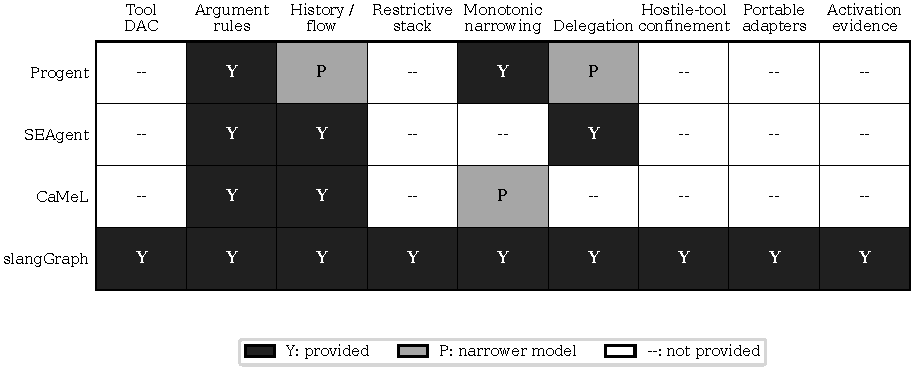
\includegraphics[width=\textwidth]{figures/expressiveness.pdf}
\caption{Qualitative comparison from the systems' published designs.
``Confine'' means enforcement below an admitted implementation, not rejection
of a proposed call. ``Narrow'' includes monotonic policy updates or semantic
argument attenuation in the system's stated model. No prior system is claimed
inferior in its own target model; the novelty is the joint column set.}
\label{fig:features}
\end{figure*}

To our knowledge, no prior agent-security framework jointly provides all nine
properties. This is our expressiveness claim: it concerns the range and
composition of enforceable authority, not automated policy inference. The
current Linux backend realizes only the filesystem/resource subset of the
portable adapter model; service adapters remain necessary for useful mail, SQL,
or remote-network grants.

\subsection{Q2: sinks below the call boundary}

We built eight intentionally vulnerable tools: file read/write, shell, SQL,
fetch, email, Slack, and delegation. Each contains one security-sensitive sink.
The analyzer traces arguments and ambient values through resource resolution,
post-validation transformations, native calls, and service operations. We score
each defense generously: a sink counts mediated whenever a sound argument
constraint could dominate every tainted path, even if the released policy omits
that constraint.

Figure~\ref{fig:exposure} reports exposed sinks. Policy-only \sys is intentionally
8/8: an authorization decision is not mislabeled as confinement. Progent
mediates the explicit delegation boundary but leaves seven implementation sinks
below its check. CaMeL's data-flow model covers the eight headline paths under
our generous untrusted-tag assumption; Section~\ref{sec:limitations} explains
why this is not a claim that CaMeL is bypassed generally. The projected \sys host
model covers local file/process effects but not semantic services; a composed
host+service+resource model covers all eight. The projected rows motivated the
adapter design and are not dynamic evidence.

\begin{figure}[t]
\centering
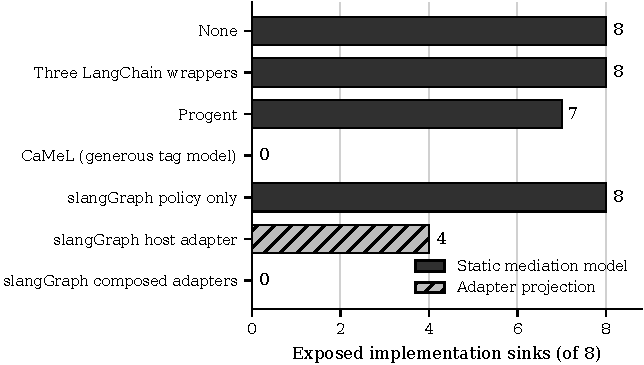
\includegraphics[width=\columnwidth]{figures/exposure.pdf}
\caption{Static E1 exposure. Projected adapter rows model capability and host
availability; they are not runtime blocking results.}
\label{fig:exposure}
\end{figure}

The deterministic E2 canaries then ask a narrower runtime question: can a
policy-conformant call reach an unauthorized implementation sink? All eight
canaries landed with no defense and after Progent approved the calls. The same
8/8 landed behind each tested generic LangChain wrapper (Eydii, Forge, and
Nuggets). A scoped CaMeL auxiliary case also landed when a value trusted at the
policy boundary became an absolute path during post-validation resolution
(1/1); this case is not comparable to CaMeL's ordinary untrusted-tag threat
model. These results establish the existence of below-boundary effects, not an
attack-success-rate comparison among complete systems.

\subsection{Q3: Linux contract and failure behavior}

The Linux milestone froze eight requirements before validation. Table
\ref{tab:acceptance} summarizes the mechanism and focused failures. The complete
unmodified \code{langgraph-prebuilt} suite passed 518 tests; a focused Linux and
flow run passed 55. Kernel-dependent claims use real bubblewrap/seccomp
integration, not a mocked adapter.

\begin{table*}[t]
\centering
\small
\begin{tabularx}{\textwidth}{clXl}
\toprule
ID & Property & Enforcing mechanism & Representative failures \\
\midrule
A1 & Authority accounting & Explicit mounts, roots, environment, descriptors, channels, and baseline grant lines & Ambient files, env., and FDs \\
A2 & Conservative lowering & Exact obligation assessment; operation-set and object-type rejection & Narrow writes, special files, nested mounts \\
A3 & Confinement first & Namespaces/mounts before Python; rlimits/seccomp before \code{GO}; deferred source compile & Imports, shadow modules, bytecode \\
A4 & Authentic activation & Challenge plus parent-observed kernel state bound to grant, plan, payload, and worker & Context, receipt, mount, artifact mismatch \\
A5 & Bounded results & 1 MiB frames; JSON-only depth/node bounds; isolated stdout/stderr & Oversize, malformed, deep results \\
A6 & Safe lifetime & Wait plus PID/start disappearance; kill on timeout; durable uncertain recovery & Timeout, cancellation, unconfirmed exit \\
A7 & Persistent flow & Atomic SQLite joins/reservations/transfers; fail-closed recovery & Crash, restart, concurrent source/sink \\
A8 & Accurate limits & Mechanism-specific names and unsupported-limit rejection & Fractional CPU, RSS, persistent quota \\
\bottomrule
\end{tabularx}
\caption{Frozen Linux acceptance contract. Each row is supported by code-path
evidence and focused tests; suite totals are corroborating rather than proof.}
\label{tab:acceptance}
\end{table*}

The validation found and fixed five classes of defect: flow reservations were
released after uncertain termination; async cancellation could outlive its
reservation; special files and nested-mount subtrees were accepted; unrestricted
\code{ioctl} exceeded the declared mutation set; and resource names overstated
CPU precision and physical-memory enforcement. These findings illustrate why
interface presence and happy-path tests are insufficient evidence.

\subsection{Q4: compatibility and policy overhead}

We ran matched \code{pytest-benchmark} cases on the same checkout and host. Each
case invokes a no-op tool through a complete synchronous \code{ToolNode}; the
only change is security configuration. Figure~\ref{fig:perf} reports overhead
relative to the security-disabled median. Capability-only mediation increases
median latency by 13.2\% (593.701 to 672.212~$\mu$s); five no-op modules increase
it by 49.0\% (to 884.800~$\mu$s). The corresponding absolute increments remain
below the 200~$\mu$s and 1~ms engineering targets. These numbers measure
in-process policy mediation, not fresh Linux worker launch.

\begin{figure}[t]
\centering
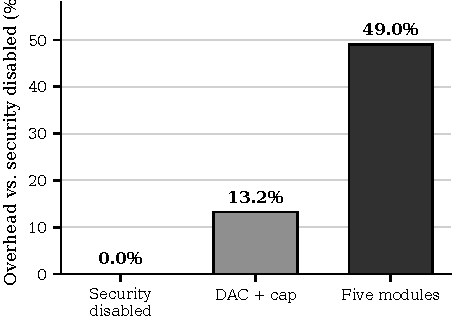
\includegraphics[width=\columnwidth]{figures/overhead.pdf}
\caption{Median policy-path overhead relative to security disabled, Python
3.12.3. Fresh-worker latency is intentionally not inferred from these
measurements.}
\label{fig:perf}
\end{figure}

With security omitted, the upstream execution path remains the default. New
request fields have defaults, and no LangChain Core class is modified. The full
suite's 518 passing tests include the unchanged upstream ToolNode tests. Released
artifact validation additionally passed CaMeL's 126 tests and three Progent
checker-parity cases; these confirm harness compatibility, not comparative
security.

\section{Discussion}

\subsection{Why an adapter abstraction matters}

A Linux mechanism is not an authorization model. If policy directly emitted
Landlock rights or bubblewrap arguments, moving to Windows would change policy
semantics and silently weaken unsupported rules. \sys instead negotiates exact
obligations against a host statement and selected adapters. A Windows backend
could use handles, restricted tokens, job objects, and filtering mechanisms;
the grant remains unchanged. A service adapter can coexist with either host.

This split also prevents a common category error: host capability is not adapter
support. The host may expose a primitive for which no trusted adapter is
selected, or an adapter may understand a rule the host cannot realize. Both are
diagnostics, not permission to approximate.

\subsection{Authorization is not intent}

Least privilege is relative to a task. A principal's maximum envelope may allow
email to a corporate recipient, yet the current user request may not authorize
that message. For consequential operations, deployments should issue
task-specific authority bound to principal, tool artifact, normalized concrete
parameters, policy version, expiry, and replay rules. Approval is such an input,
not an override of unconditional denial. \sys enforces issued authority; it does
not claim to infer the correct authority from natural language.

\subsection{Deployment choices}

Fresh workers maximize boundary clarity but add launch cost. Preinitialized
workers would need to remain free of untrusted imports, prove clean state, and
bind each activation to a new grant. Long-lived workers complicate revocation,
flow reservations, and dependency state. We therefore choose fresh workers for
the reference implementation and leave pooling as an adapter-specific
optimization subject to the same contract.

\section{Limitations}
\label{sec:limitations}

The current Linux backend is intentionally incomplete in authority domains.
Useful network, mail, SQL, cloud, and credential-bearing tools require trusted
service/resource adapters; today such grants deny. This produces security by
refusal, not useful least-privilege execution. We therefore do not present the
static composed-adapter projection as an implemented result.

The accepted contract protects mediated tool workers, not the entire graph
process. A trusted callback can still become a confused deputy by interpreting
tool output. Model inference, tracing, telemetry, rendering, checkpoints, and
artifact handlers must be mediated sinks or explicitly trusted destinations.

Session-flow scheduling relies on operator-complete labels and mediated
transfers. It does not track arbitrary dependencies through model context or
shared external artifacts. Siblings can pool authority through any unmediated
channel. The Linux no-process profile bounds background descendants, but the
trusted in-process path does not supervise them.

Activation evidence is local and software-rooted. It does not protect against a
compromised kernel, bubblewrap, seccomp library, launcher, policy backend, or
trusted module. Read-only mounts do not make backing objects immutable, and live
subtrees permit external mutation. The primary tool source is digest-pinned;
dependency identity is not.

Our comparative E1 analysis is small and synthetic. Static exposure is an upper
bound; E2 canaries establish particular lower-bound bypasses. The completed
artifact does not yet contain dynamic \sys runs over AgentDojo, InjecAgent, or
ASB, nor a fresh-worker latency distribution. Those experiments are necessary
before a final empirical claim about benchmark utility or deployment overhead.

\section{Related Work}

\paragraph{Agent policy and information flow.}
Progent expresses symbolic privilege rules over tool names and arguments and
uses SMT to ensure unapproved policy updates only shrink authority~\cite{progent}.
SEAgent models multi-agent privilege escalation using ABAC and an information-
flow graph~\cite{seagent}. CaMeL separates trusted control flow from untrusted
data and applies capabilities to prevent unauthorized flows~\cite{camel}. These
systems motivate our argument policy, history, and monotonicity. \sys differs by
making the tool's DAC, independent mandatory modules, host/service/resource
lowering, and activation evidence one framework contract. Its flow scheduler is
coarser than CaMeL and explicitly conditional on confinement and complete labels.

\paragraph{Agent-security benchmarks.}
AgentDojo provides stateful tasks and security cases for indirect prompt
injection~\cite{agentdojo}. InjecAgent contains 1,054 cases over user and attacker
tools~\cite{injecagent}; ASB spans multiple attack classes, agents, scenarios,
and hundreds of tools~\cite{asb}. These benchmarks primarily score behavioral
attack success and utility. Our exposure census instead asks whether effects lie
below a defense's mediation point. The measures are complementary.

\paragraph{Security frameworks and sandboxing.}
LSM's fixed hooks, preserved DAC, module stacking, and opaque per-object state
directly inspire \sys~\cite{wright2002lsm}. Prior work also showed that hook
placement itself requires systematic analysis~\cite{zhang2002cqual}. Landlock
lets unprivileged processes add filesystem restrictions and composes
restrictively with existing controls~\cite{landlock}; bubblewrap constructs
namespace/mount sandboxes for unprivileged workloads~\cite{bubblewrap}. \sys is
not tied to either mechanism: these are possible Linux implementations behind a
semantic adapter contract.

\paragraph{Authorization languages.}
Cedar offers typed, analyzable principal--action--resource--context policies and
permit-overridden-by-forbid composition~\cite{cedar}. \sys uses a constructive
profile language for tool/principal intersection and a typed forbid IR for
mandatory modules. A Cedar backend can implement mandatory filtering, but native
enforcement plans remain outside Cedar.

\section{Conclusion}

Agent security cannot stop at deciding whether a tool call looks acceptable.
For hostile implementations, the security property lives below that interface:
actual authority must be no broader than an exact grant, every restriction must
have an enforcer, and the system must know that enforcement was active for the
worker that ran.

\sys brings this principle into LangGraph through LSM-style hooks, constructive
DAC, restrictive mandatory modules, platform-neutral grants, exact obligation
negotiation, and verified activation. Its Linux backend demonstrates a working
filesystem/resource boundary with conservative failure semantics. The result is
not automatic agent safety. It is a precise foundation on which independently
authored policies and replaceable enforcement mechanisms can compose without
turning unsupported authority into an implicit allow.

\bibliographystyle{plain}
\bibliography{references}

\appendix
\section{Open Science}

The anonymized artifact will include the LangGraph fork, the standalone
evaluation harness, pinned dependency manifests, deliberately vulnerable tools,
frozen model transcripts, hash-chained audit databases, generated tables, and
commands for reproducing E0--E2, the Linux acceptance suite, and policy
microbenchmarks. At submission, this paragraph will contain a history-free,
non-tracking SEC27 artifact URL. The public repository and author-identifying
commit history are intentionally omitted during double-blind review.

The artifact distinguishes measured data, static projections, and pending work
in machine-readable reports. Third-party source is pinned but remains under its
original license. Runs that require unavailable hosted models are not silently
substituted; local-model settings and immutable layer digests are recorded.

\section{Ethical Considerations}

This work studies defenses for attacker-influenced agents. The bypass examples
could help identify weak call-boundary guards, but require no novel exploit
against a deployed service. Dynamic experiments target only deliberately
vulnerable tools in temporary directories, loopback listeners, and synthetic
data. We do not probe or modify third-party deployments. Canary values are fake,
and audit logs hash arguments by default.

The framework can be misconfigured to deny legitimate work or to create a false
sense of confinement. We mitigate this risk by rejecting unsupported grants,
labeling degraded results, publishing a frozen threat model, and separating
interface decisions from enforcement evidence. Operators remain responsible for
policy correctness, TCB maintenance, user notice, and recovery from
\code{INDETERMINATE} operations.

\section{Artifact Evidence Map}

The anonymous snapshot preserves the following claim-to-evidence map:

\begin{itemize}
  \item Linux A1--A8: the frozen contract, execution path, defects, and focused
  tests in \path{docs/security/linux-enforcement-acceptance.md}.
  \item Compatibility: run \code{make test} from \path{libs/prebuilt}.
  \item Policy overhead: \path{benchmarks/test_tool_node.py} and
  \path{benchmarks/test_security_overhead.py}.
  \item Static exposure: per-sink traces and mediation decisions in
  \path{eval/reports/e1/exposure.json}.
  \item Runtime canaries: replayed calls and observed local side effects in
  \path{eval/reports/e2/}.
  \item Third-party parity: released suites and checker comparisons in
  \path{eval/reports/generated/e0-baseline-validation.md}.
  \item Reproducibility: hardware, model, source, and package identities in
  \path{eval/HARDWARE.md} and \path{eval/PINS.md}.
\end{itemize}

\end{document}
